%%%%%%%%%%%%%%%%%%%%%%%%%%%%%%%%%%%%%%%%%%%%%%%%%%%%%%%%%%%%%%%%%%%%%%%%%%%%%%%%%%%%%%%%%%%%%%%%%%%%
% ==================================================================================================
% --------------------------------------------------------------------------------------------------
\chapter{Pre-Processing}\label{ch-pre}
The proposed VLR classification model addresses
several of the challenges outlined in \S~\ref{ss:autochallenges}.
The problem of overlapping tissue graylevel distributions
is mostly solved through expansion of the feature space to include spatial features.
CSF flow-through artifacts, which appear in roughly consistent locations, are similarly managed.
Heterogeneity in the appearance of lesions is also considered
by the spatial parametrization of logistic parameters.
Finally, ambiguity regarding moderately hyperintense DAWM,
and voxels affected by partial volume effect,
is captured in the probabilistic output.
\par
Several challenges, however, still remain.
In particular, a number of assumptions were made about the input data for the VLR model
which are likely invalid for raw images.
These assumptions are that:
1.\ input MRI images are free of bias field artifact;
2.\ feature intensities are consistent across different subjects;
3.\ images are consistently sized and
voxels represent the same anatomical regions across different subjects.
Solving these challenges must therefore be accomplished by one or more pre-processing steps.
This section explores these steps.
%%%%%%%%%%%%%%%%%%%%%%%%%%%%%%%%%%%%%%%%%%%%%%%%%%%%%%%%%%%%%%%%%%%%%%%%%%%%%%%%%%%%%%%%%%%%%%%%%%%%
\section{Registration}\label{s:pre-reg}
Image registration is the process of geometrically transforming a source image
so that the image content is aligned per-voxel with a target image of the same subject.
This process facilitates voxel-wise analysis of MRI from different subjects,
such as  ``voxel-based morphometry''~\cite{Ashburner2000a}
and analysis of functional MRI data~\cite{Smith2004}.%
\footnote{Incidentally, investigation of these topics were the motivations
  for developing of the SPM and FSL software packages, respectively.}
Source images from multiple subjects are usually registered to the same target image; 
in this context, it is useful to define a ``native space'' and a ``standardized space'',
denoting the original, subject-specific geometry, and the standardized target geometry.
By convention, the target brain space is usually either
the Talairach space~\cite{Talairach1988} or
the Montreal Neurological Institute (MNI) space~\cite{Evans1993},
though any reasonable target image could be used.
Figure~\ref{fig:pre-registration} shows three FLAIR images before and after registration,
with cross-hair shown to highlight differences in alignment corrected by the transformation.
\par
\begin{figure}
  \centering
  \subfigureoverl[white]{(a) Native Space}{}{%
    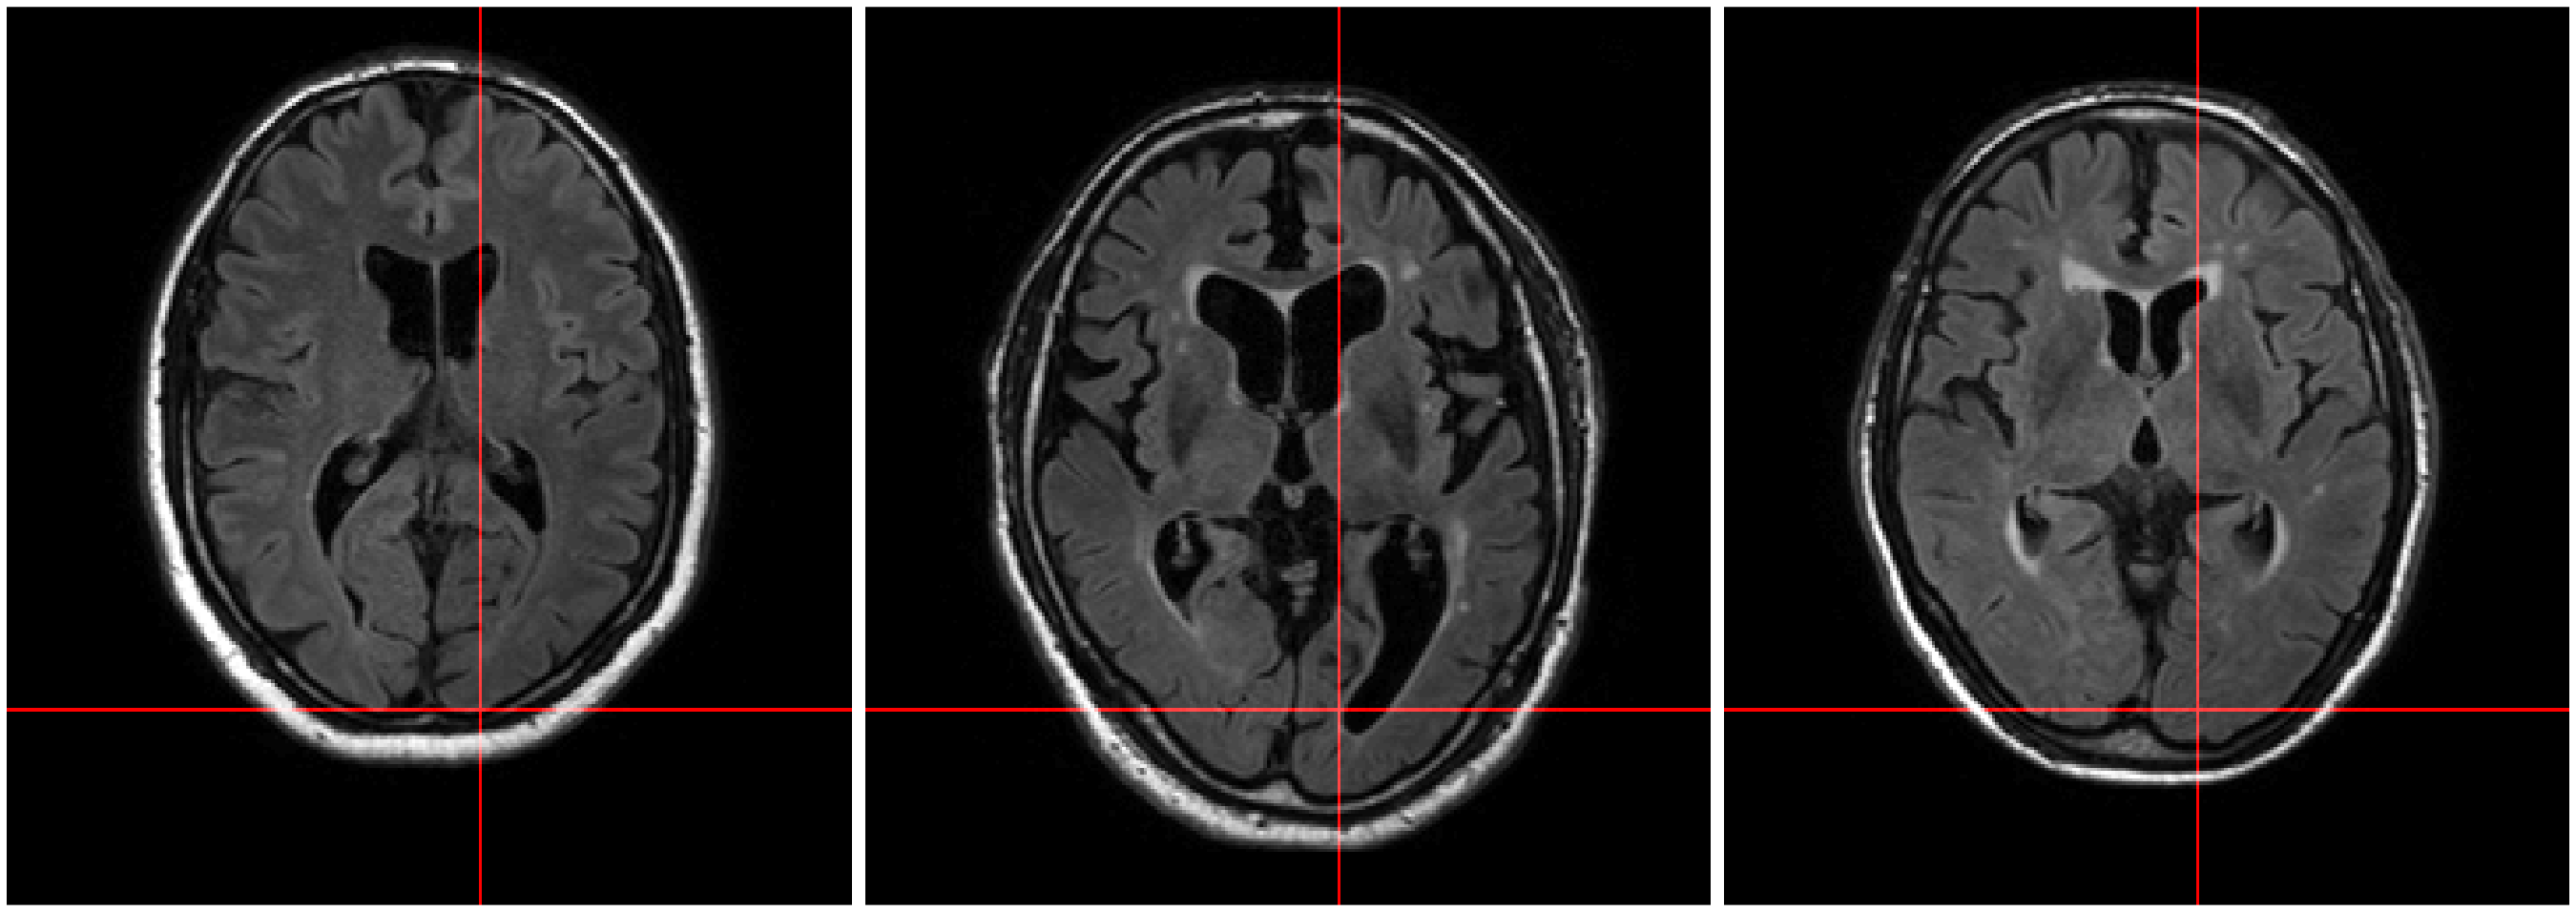
\includegraphics[width=0.9\textwidth]{pre-registration-1.png}
  }\\[0.5em]
  \subfigureoverl[white]{(b) Standard Space}{}{%
    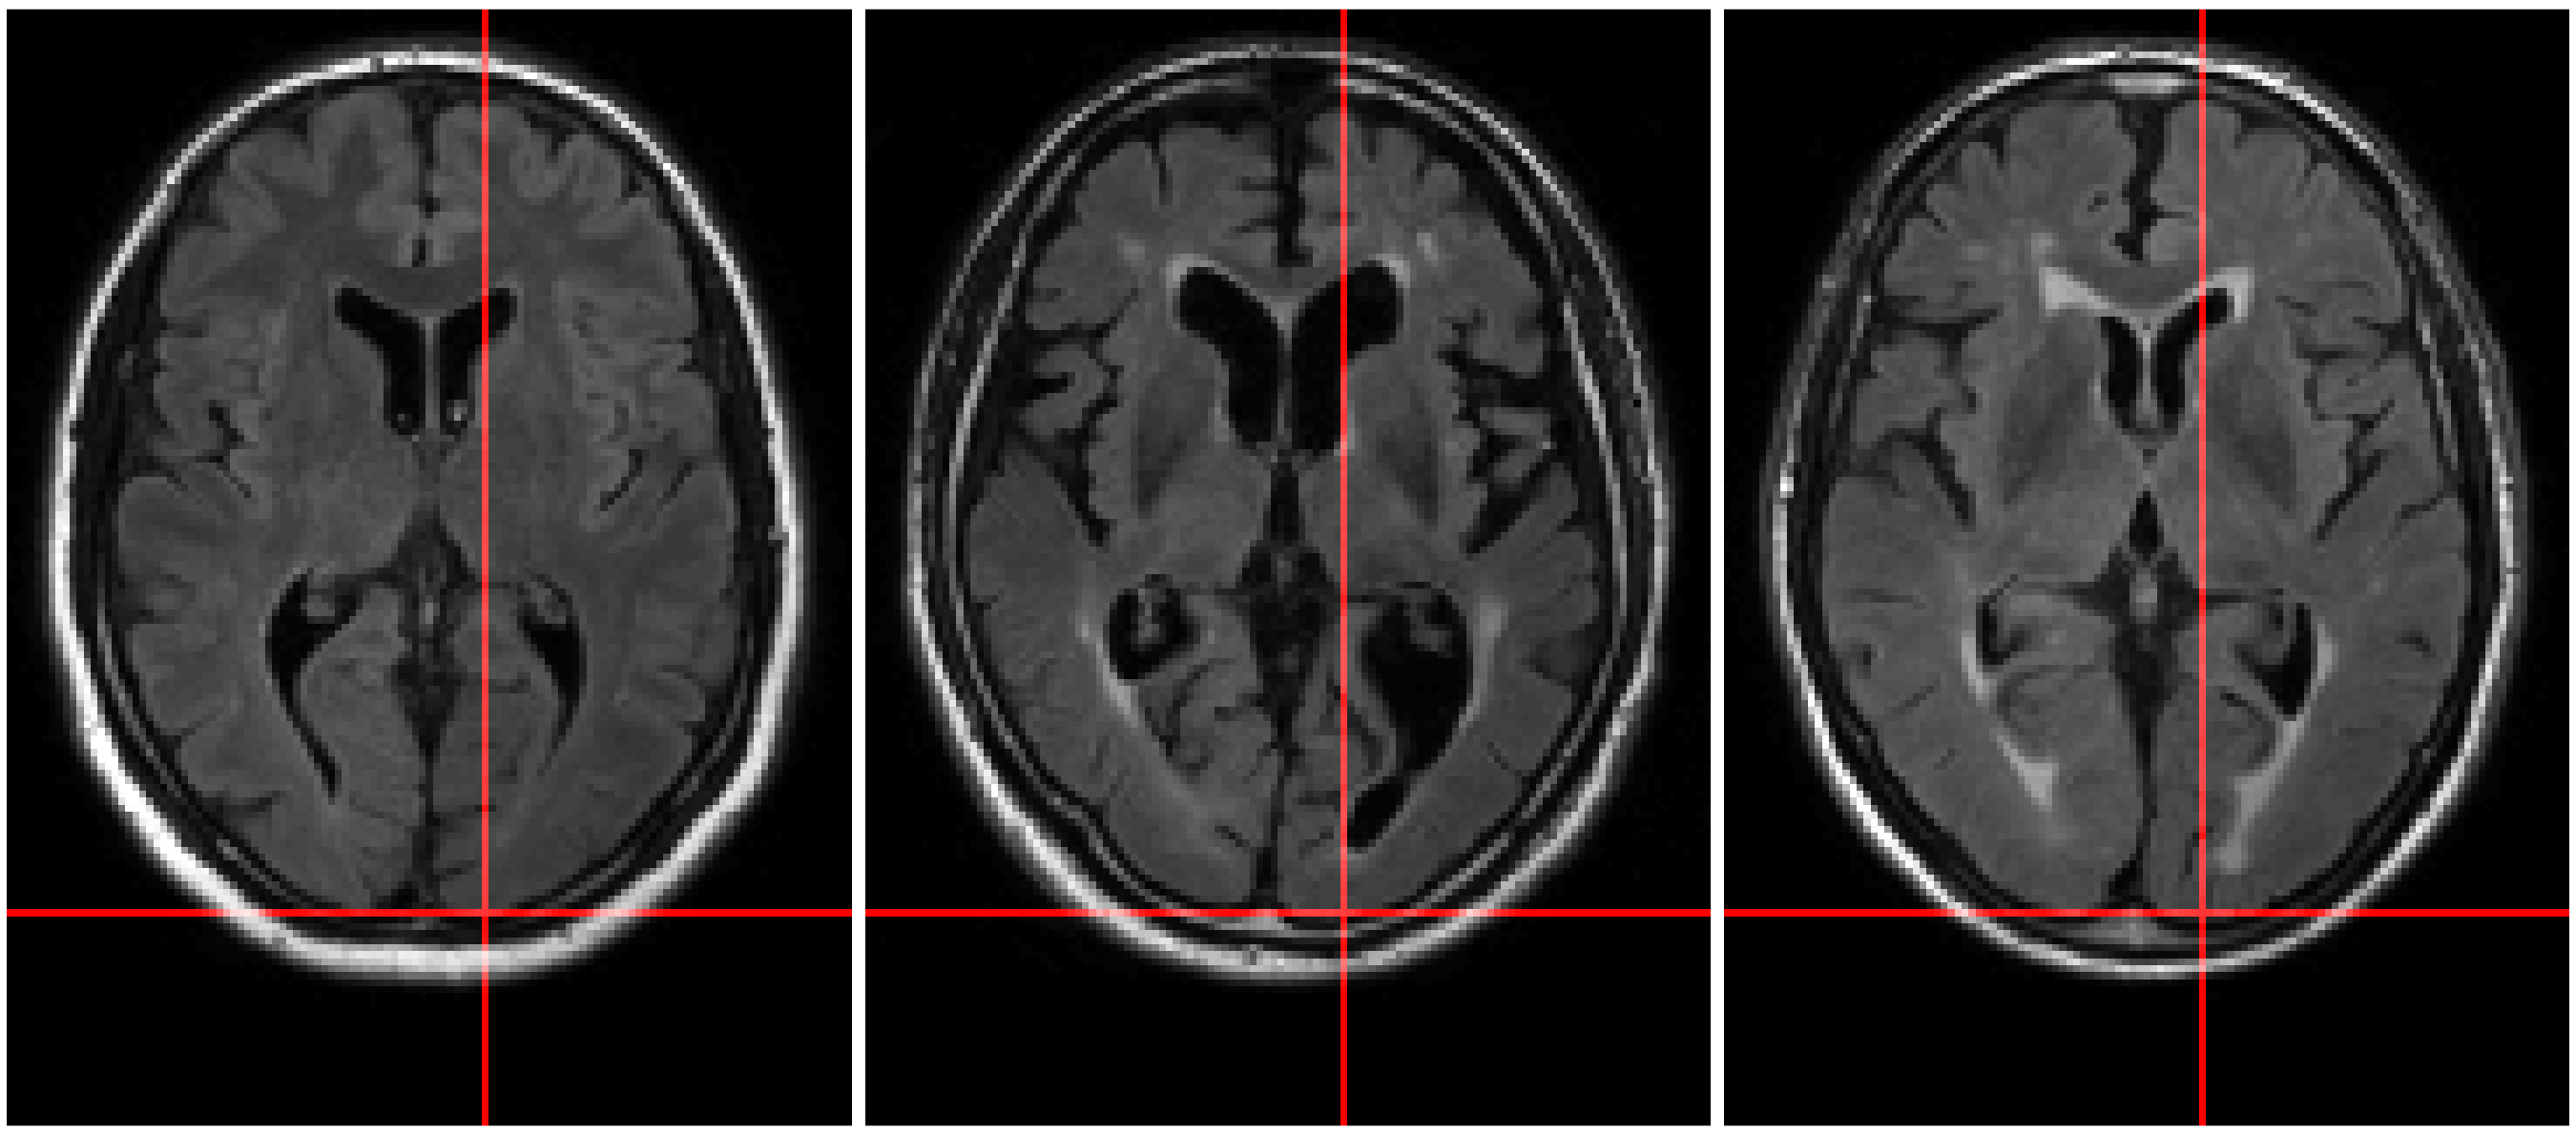
\includegraphics[width=0.9\textwidth]{pre-registration-2.png}
  }
  \caption{Example set of FLAIR MRI before and after registration to the MNI brain space.
    From~\cite{WMHSEG2017}.}%
  \label{fig:pre-registration}
\end{figure}
Parameters defining registration transforms are fitted by
maximizing some measure of overlap between the images~\cite{Sotiras2013}.
Simple registration methods employ only affine transformations,
comprising a combination of translation, scaling, and shear transformations
(e.g.\ the FLIRT tool~\cite{Jenkinson2002} in FSL).
The utility of these methods for neuroimage analysis is limited,
since there are often significant differences in brain anatomy between subjects.
Rather, most tools parametrize a spatial warping model,
permitting local nonlinear deformations to better match brain structures (e.g.\ 
cubic B-splines in FSL FNIRT~\cite{Andersson2007},
discrete cosine transform in SPM Normalize~\cite{Ashburner1997,Ashburner2005},
a general diffeomorphism in the SyN algorithm~\cite{Avants2008}).
While these models are more difficult to fit,
several robust algorithms have been released for general use,
with widespread acceptance (e.g.\ the toolboxes mentioned above).
A~\citeyear{Klein2009} comparison of 14 different methods
is a good resource on the subject~\cite{Klein2009},
while a more recent (\citeyear{Kazemi2014}) study
ranks the popular toolboxes SPM, FSL, and Brainsuite~\cite{Kazemi2014}.
\par
In the current work, registration is required during both training at testing.
During training, the model parameters $\bb(x)$ are estimated using
mutually aligned segmentation examples $\{\bY,\C\}$ in a standard brain space.
At test time (or for actual use), these parameter images
are transformed in the opposite direction from the standard space
to the native space of the current subject.
Since registration transforms are typically bijections -- i.e.\ invertible --
the second registration case can be estimated using the same method as the first, minimizing bias.
\par
Unlike other applications, it is not essential that perfect image registration is achieved here.
As noted by~\citeauthor{Harmouche2015}~\cite{Harmouche2015}, in smoothly varying models,
small registration errors can be expected to have a negligible impact.
Therefore, registration was not a primary focus of optimization in this work.
\par
While the registration component of the SPM8 ``Segment'' feature~\cite{Ashburner2005}
was not among the top performing in the~\citeyear{Klein2009} study~\cite{Klein2009},
subsequent implementation revisions in SPM12%
\footnote{\hreftt{http://www.fil.ion.ucl.ac.uk/spm/software/spm12/SPM12_Release_Notes.pdf}}
called ``New Segment'' have apparently improved results.
In the~\citeyear{Kazemi2014} study~\cite{Kazemi2014}, the SPM12 New Segment method
achieved the highest Similarity Index of all methods on real (IBSR~\cite{IBSR}) data.
\par
Furthermore, the SPM module has several other features amenable to this work.
First, unlike many other registration algorithms,
the objective function does not require source and target images to have the same contrast.
This is helpful, since no suitable FLAIR template image is available for use as a target.%
\footnote{One FLAIR template is available in~\cite{Winkler2012};
  however, this was generated using SPM5, so using it
  would compound any registration biases associated with the older method.}
Second, it is simple to invoke the SPM modules via the command line or Matlab scripts;
this facilitates smooth integration of this tool in the pipeline.
Third, it is possible to save previously estimated registration transformations,
and apply them in the forward or reverse directions efficiently.
This can save significant time during cross validation,
since the estimated parameter images $\bm{\b}(x)$ must eventually be transformed
to the native space of every subject.
Finally, the SPM ``New Segment'' model additionally estimates the bias field during execution
with high accuracy, saving an additional step (cf.~\S~\ref{s:pre-bias}, below). 
For all these reasons, the registration performed by SPM New Segment was used throughout this work.
After satisfactory visual inspection of all training set images,
no other registration tools were investigated.
The default brain space of this module is MNI.
%%%%%%%%%%%%%%%%%%%%%%%%%%%%%%%%%%%%%%%%%%%%%%%%%%%%%%%%%%%%%%%%%%%%%%%%%%%%%%%%%%%%%%%%%%%%%%%%%%%%
\section{Bias Correction}\label{s:pre-bias}
As noted in \S~\ref{ss:autochallenges}, bias field (\textsc{aka} intensity inhomogeneity),
is a smoothly varying intensity variation artifact common in MRI.
The sources of bias field artifact include
inhomogeneities in the magnetic field and RF coils used for pulse transmission and signal sensing,
as well as non-ideal magnetic properties of the imaged object~\cite{Vovk2007}.
The field and coil related sources are more significant at clinical field strengths.
These can be corrected prospectively, though techniques for doing so are limited,
and often a small bias field continues to corrupt acquired images~\cite{Vovk2007}.
Therefore, retrospective correction has been the subject of much research.
\par
Similar to image registration,
several widely accepted algorithms for estimating and correcting bias field have emerged.
The N3 algorithm~\cite{Sled1998}, subsequently updated to N4(ITK)~\cite{Tustison2010}
and integrated in the FreeSurfer toolbox%
\footnote{\hreftt{https://surfer.nmr.mgh.harvard.edu/}}
is perhaps the most popular, it makes minimal assumptions about the image.
This method aims to sharpen the image histogram by dividing the image by an estimated bias field,
parameterized by B-splines for smoothness.
As noted above, the SPM Segment model~\cite{Ashburner2005} 
includes integrated bias field estimation and correction.
The bias field model in this work is parameterized by the discrete cosine transform,
as described in in a previous work by~\citeauthor{Ashburner2005}~\cite{Ashburner1999}.
The FSL Segment feature also estimates bias field in a similar overall model to SPM Segment,
except the tissue prior probability maps in SPM are replaced with a Markov Random Field Model,
as described in~\cite{Zhang2001}.
Again, two reviews with quantitative performance comparisons
provide a good reference of other proposed algorithms,
including a comprehensive review in~\citeyear{Belaroussi2006}~\cite{Belaroussi2006}
and a comparison of mainly popular methods in~\citeyear{Ganzetti2016}~\cite{Ganzetti2016}.
\par
In the~\citeyear{Ganzetti2016} comparison~\cite{Ganzetti2016},
the authors note that the SPM and FSL models -- which include segmentation --
outperformed the N3 algorithm~\cite{Sled1998} and another non-segmenting method~\cite{Dawant1993}.
These results are consistent with
the advantages of unified generative models described in \S~\ref{sss:prior-models}
and discussed in~\citetitle{Ashburner2005}~\cite{Ashburner2005}.
Specifically, the estimation of both bias field and tissue segmentation are each improved
if the other is already known.
Rolling these tasks into a single EM-fitted model allows
alternating conditional estimates to converge on better results overall.
\par
Bias field estimation was not a primary focus of this work.
Therefore, due to the better performance over N3/4,
and the advantages already afforded by SPM Segment for registration noted above,
this model was employed for bias correction throughout this work.
No other bias field correction tools were investigated.
Figure~\ref{fig:pre-bias} shows a FLAIR image with conspicuous bias field,
the bias field estimated by SPM, and the corrected image.
\par
% could use another couple references here...
\begin{figure}
  \centering
  \begin{subfigure}{0.3\textwidth}
    \centering
    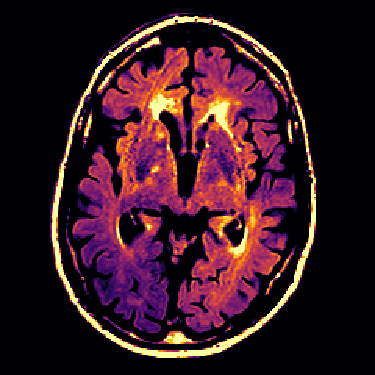
\includegraphics[height=1.5\sliceheight]{pre-bias-1.png}
    \caption{Raw FLAIR}
  \end{subfigure}
  \begin{subfigure}{0.3\textwidth}
    \centering
    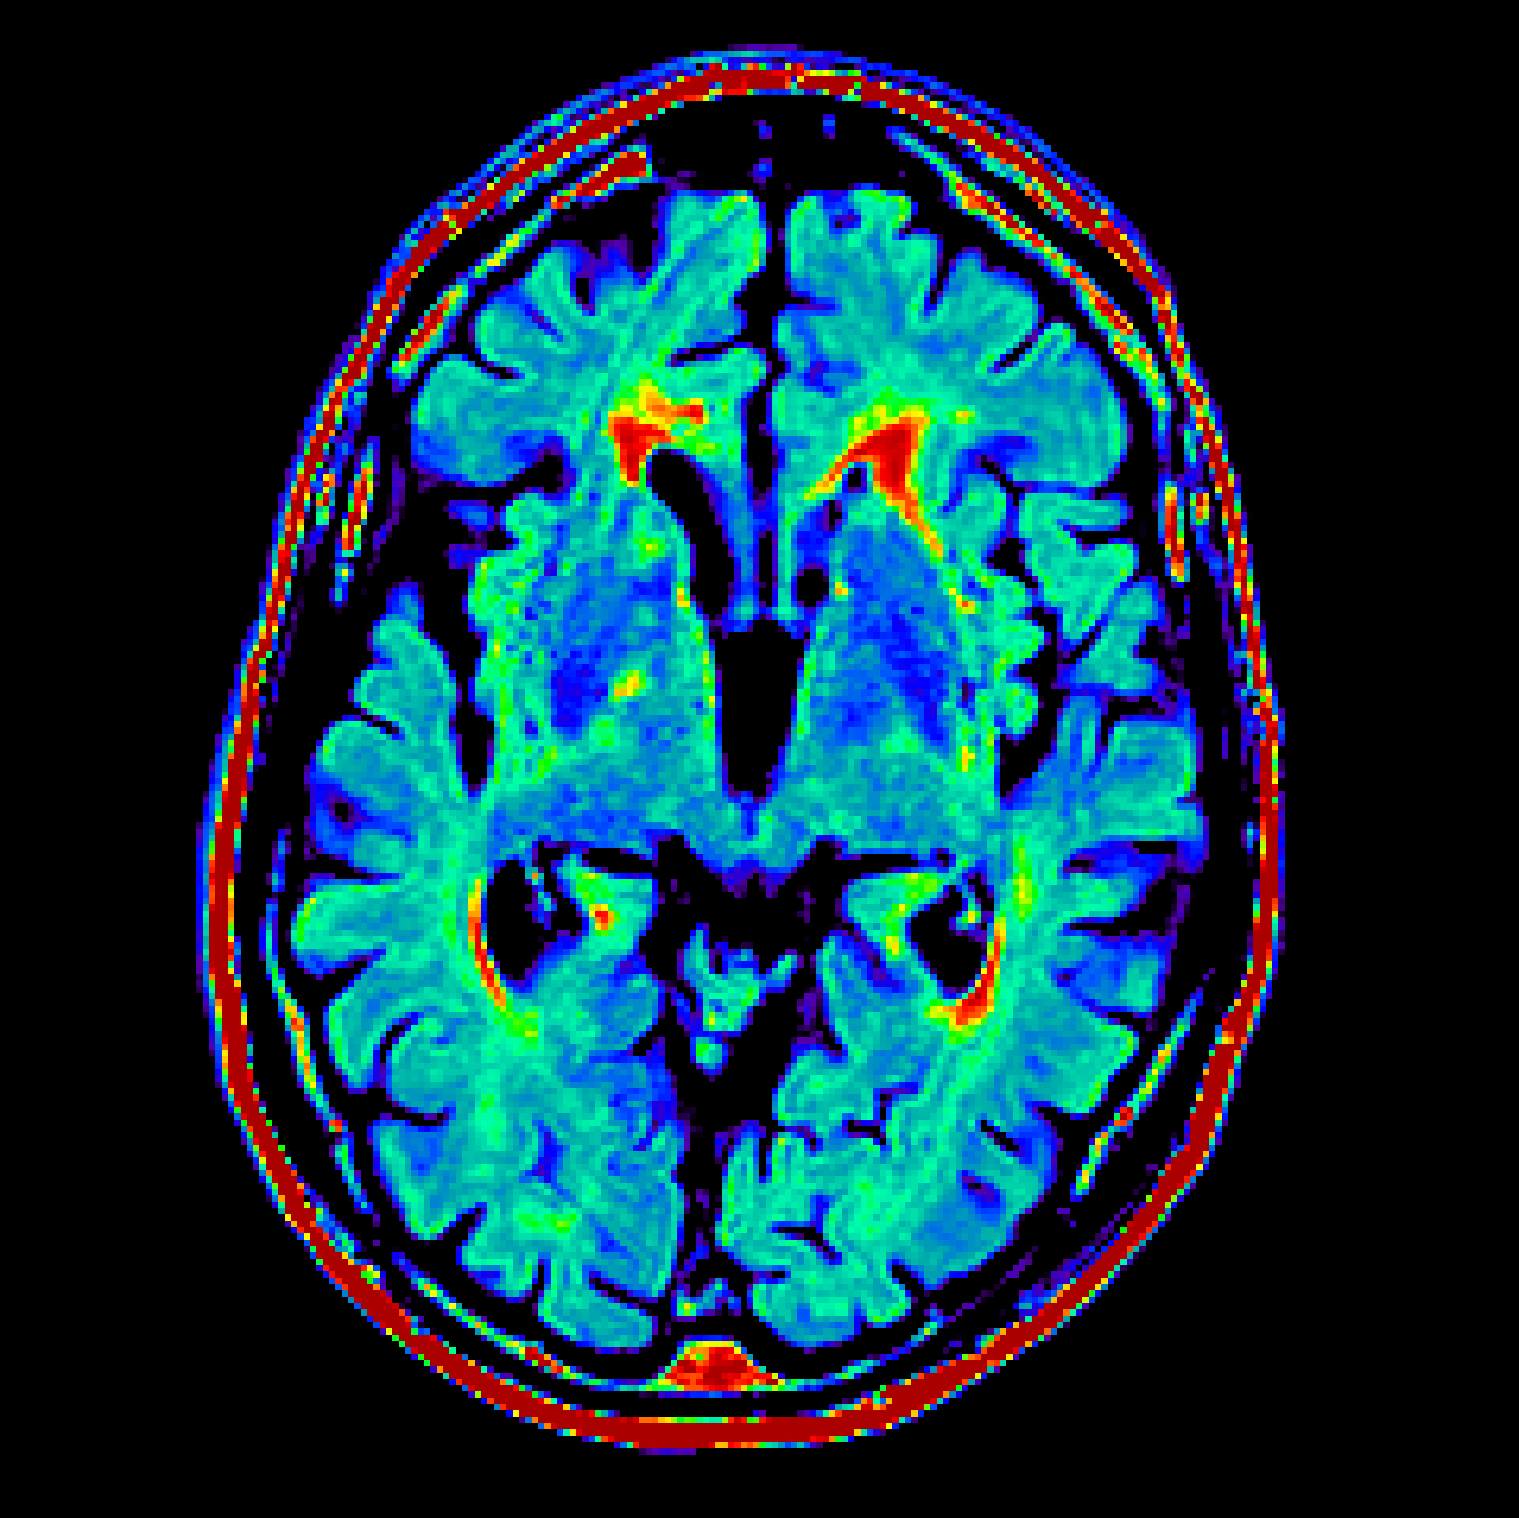
\includegraphics[height=1.5\sliceheight]{pre-bias-2.png}
    \caption{Bias-corrected FLAIR}
  \end{subfigure}
  \begin{subfigure}{0.30\textwidth}
    \centering
    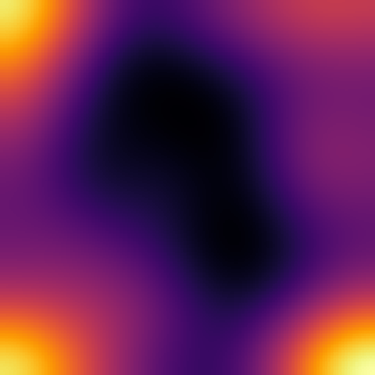
\includegraphics[height=1.5\sliceheight]{pre-bias-3.png}
    \caption{Estimated bias field}
  \end{subfigure}
  \begin{subfigure}{0.04\textwidth}
    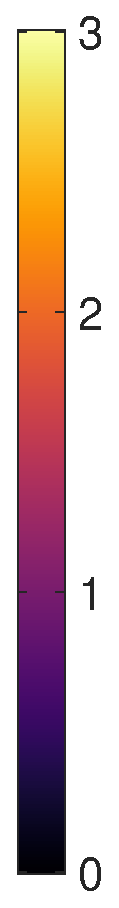
\includegraphics[height=1.5\sliceheight]{cmap-pre-bias}
    \\\vphantom{(x)}
  \end{subfigure}
  \caption{Example bias correction. From~\cite{WMHSEG2017}.}%
  \label{fig:pre-bias}
\end{figure}
%%%%%%%%%%%%%%%%%%%%%%%%%%%%%%%%%%%%%%%%%%%%%%%%%%%%%%%%%%%%%%%%%%%%%%%%%%%%%%%%%%%%%%%%%%%%%%%%%%%%
\section{Graylevel Standardization}\label{s:pre-ystd}
The flexibility of image contrast in MRI is a double-edged sword.
This feature, in addition to properties of spatial encoding during acquisition,
preclude direct interpretation of image graylevels as a tissue property.
As a result, the same brain region in the same subject may be assigned a different graylevel
depending on the MRI sequence time constants, scanner, and spatial acquisition protocol.
For automated analysis of MRI images, therefore, standardization of image graylevels is required.
\par
Graylevel standardization can be achieved using a univariate transformation
$\uptau:y\mapsto\tilde{y}$, defined as
\begin{equation}
\tilde{y} = \uptau(y),
\end{equation}
where $\uptau$ is monotonic, and considers characteristics of the input image,
such as basic graylevel statistics or the histogram.
The histogram of an image represents the number of occurrences of each graylevel in the image.
Normalizing the histogram by the total number of voxels $X$
yields the the probability mass function (PMF) $f_{\sy}(y)$,
\begin{align}
f_{\sy}(y) &= \frac{1}{X}h_{\sy}(y)\nonumber\\
&= \frac{1}{X}\sum_{i=1}^{X}
\begin{cases}
1&Y(x_i) = y\\
0&Y(x_i) \ne y\\
\end{cases}
\end{align}
The cumulative density function (CDF) $F_{\sy}(y)$ is the cumulative sum of $f_{\sy}(y)$,
\begin{equation}
F_{\sy}(y) = \sum_{\gamma=y_{\min}}^{y} f_{\sy}(\gamma)
\end{equation}
The PMF of an MRI can be decomposed into the contributions of each constituent tissue,
as shown in Figure~\ref{fig:simflairplot}.
This is the fundamental principle underlying mixture models (cf.~\S~\ref{ss:priorproposed}).
The goal of standardization is therefore to align these sub-distributions as closely as possible.
\par
Previously proposed methods of standardizing MRI intensities include the following:%
\footnote{This section considers only univariate standardization methods,
  since only FLAIR intensities are used in this work.}
\begin{itemize}
  \item \textbf{Range Matching:}
  The simplest approach to standardization involves
  rescaling the data using the minimum and maximum intensities,
  \begin{equation}
    \uptau(y) = \frac{y-y_{\min}}{y_{\max}-y_{\min}}.
  \end{equation}
  Naively, this method is very susceptible to corruption by outliers.
  For more robustness, $y_{\min}$ and $y_{\max}$ can be defined using intensity quantiles
  -- e.g.\ $[\epsilon_1,1-\epsilon_2]$.
  However, selection of an appropriate $\epsilon_2$ for WMH segmentation is difficult,
  since WMH typically constitute only the top 1\% of the total brain volume.
  Furthermore, differences in image contrasts are not considered by this approach.
  \item \textbf{Statistical standardization:}
  Another simple but popular approach uses the first and second order moments of the PMF,
  \begin{equation}
    \uptau(y) = \frac{y-\mu_{\sy}}{\sigma_{\sy}}.
  \end{equation}
  As with range matching, variable image contrasts are not well modelled by this method.
  \item \textbf{Histogram equalization:}
  Histogram equalization transforms the image PMF to a uniform distribution,
  thereby distributing image intensities equally across the available range.
  The desired transform  is defined as the CDF of the input image
  (cf.~\cite{Gonzalez2006} for derivation),
  \begin{equation}
    \uptau(y) = F_{\sy}(y).
  \end{equation}
  The chief assumption of histogram equalization for standardization is
  that input images contain consistent amounts of each tissue class.
  In MRI with WMH, this assumption may not be valid;
  however, this technique may still have value.
  \item \textbf{Histogram matching:}
  Histogram matching is similar to histogram equalization, except that
  the output PMF is not uniform, but some other specified distribution, $f_{\tilde{\sy}}$.
  This transform is defined as
  the function composition of the input CDF and the inverse target CDF,
  \begin{equation}
    \uptau(y) = {F_{\tilde{\sy}}}^{-1}\big(F_{\sy}(y)\big)
  \end{equation}
  While histogram matching yields images with different contrast characteristics than
  histogram equalization, these two methods are equivalent in their ability
  to standardize image graylevels
  (cf.~\ref{ss:hm-vs-he} for an illustration and experimental evidence).
  \item \textbf{Nyul standardization:}
  In~\cite{Nyul1999,Nyul2000},~\citeauthor{Nyul1999} proposed a method for
  intensity standardization which has subsequently been used in other works. %__JK__find these
  This method defines $\uptau$ with piecewise linear segments
  connecting the $Q$ quantiles of the input PMF $q$, with quantiles of a target PMF $r$,
  \begin{equation}
    \uptau(y) = r_i + \left(y-q_i\right)
      \left(\frac{r_{i+1}-r_i}{q_{i+1}-q_i}\right),\quad y\in[q_i,q_{i+1}]
    \end{equation}
  However, it can be shown that this transformation is
  a non-uniform trapezoidal Riemann approximation of true histogram matching,
  which performs worse in terms of intensity standardization.%
  \footnote{This result is presented and supported with experiments in~\cite{Knight2017}.} % chktex 42
  \item \textbf{Regional characteristics:}
  Decorrelating variation in intensities from variability in anatomical content
  is a central challenge in intensity standardization.
  One solution is to define the image-specific transformation using characteristics
  from a more anatomically consistent brain region.
  This is the approach employed by~\citeauthor{Shinohara2014}
  in the so-called white stripe method~\cite{Shinohara2014}.
  In the current work, this region, denoted $\X_{\uptau}$,
  can be defined in MNI space using tissue priors (Figure~\ref{fig:tpm-3}),
  anatomical label maps, or any other method of selecting a subset of voxels.
\end{itemize}
% ==================================================================================================
\subsection{Quantifying Standardization}
While the major advantages and challenges to several graylevel standardization methods
have been briefly noted, it remains to explore the utility of each experimentally.
In the current work, the goal of this step is to maximize the separation of the two classes.
This can even be maximized voxel-wise, due to the characteristics of the VLR model.
Therefore, an intermediate objective function $\Z$ should be defined
which quantifies the degree of separation of the two classes.%
\footnote{Alternatively, the entire pipeline can be executed under cross validation
  and overall performance compared between standardization methods.
However this does not consider potential interactions
between the standardization method and tunable downstream parameters.}
This objective function can then be used to optimize
any tunable parameters in each of the transforms
-- e.g.\ $\bm{\epsilon}$, $Q$, $\X_{\uptau}$ -- 
and also to select the best overall method.
\par
Two such functions are proposed.
The first is discrete, and inspired by the Zero-Crossing Rate~\cite{Kedem1986}.
It measures the number of class transitions in the sorted feature data $\tilde{\Y}_s$,
as shown in Figures~\ref{fig:jsep-diff-1} and~\ref{fig:jsep-diff-2}.
With $\C_s$ as the class labels after sorting by the feature $\tilde{\Y} = \uptau(\Y)$,
the objective function $\Z_{\Delta}$ is defined as
\begin{equation}
  \Z_{\Delta} = \sum_{n=1}^{N-1}
     \begin{cases}
      1 & \C_s^{n} \ne \C_s^{n+1}\\
      0 & \C_s^{n}  =  \C_s^{n+1}
    \end{cases}.%
    \label{eq:zsep-diff}
\end{equation}
This function is discrete and bounded, as in
$\Z_{\Delta}\in\mathbb{Z}\left[1,\lfloor\frac{N}{2}\rfloor\right]$%
\footnote{The lower bound can be zero if one class is not observed.}
and the lower bound is optimal -- i.e.\ $\Z_{\Delta}$ should be minimized.
\par
The second function is continuous, and inspired by probability theory.
It measures the relative overlap of class distributions,
$p(\tilde{y}\mid c=1)$ and $p(\tilde{y}\mid c=0)$,
estimated using kernel smoothing,
as shown in Figures~\ref{fig:jsep-conv-1} and~\ref{fig:jsep-conv-2}.
This objective function $\Z_{\star}$ can be defined as
\begin{equation}
  \Z_{\star} = \int_{\tilde{y}_{\min}}^{\tilde{y}_{\max}}
    \frac{\min\{p(\psi \mid c=1), p(\psi \mid c=0)\}}
         {\max\{p(\psi \mid c=1), p(\psi \mid c=0)\}}\d\psi,
    \qquad p(\psi \mid c)
      \approx \sum_{\tilde{y}\in\{\tilde{\Y}\mid c\}}\delta(\psi-\tilde{y}) \star G_{\sigma}(\psi)%
      \label{eq:zsep-conv}
\end{equation}
where $G_{\sigma}(\psi)$ is a Gaussian convolution kernel with width $\sigma$.
This function is continuous and bounded, as in
$\Z_{\Delta}\in\left[0,1\right]$,
and the lower bound is again optimal.
\par
\begin{figure}
  \centering
  \foreach \i/\desc in {% % chktex 1
    1/{with overlapping classes},%
    2/{with barely separable classes},%
    3/{with easily separable classes}%
  }{%
    \begin{subfigure}{\plotwidth}
      \includegraphics[width=\textwidth]{jsep-diff-\i}
      \caption{$\Z_{\Delta}$ \desc}%
      \label{fig:jsep-diff-\i}
    \end{subfigure}
    \begin{subfigure}{\plotwidth}
      \includegraphics[width=\textwidth]{jsep-conv-\i}
      \caption{$\Z_{\star}$ \desc}%
      \label{fig:jsep-conv-\i}
    \end{subfigure}
  }
  \caption{Illustration of potential separability objective functions.}%
  \label{fig:jsep}
\end{figure}
% ==================================================================================================
\subsection{Supervised Standardization}
It is not hard to see that it should be possible to estimate an
optimal graylevel standardization transform using the training data.
That is, a \textit{supervised graylevel standardization}.%
\footnote{To the best of this author's knowledge, such a technique has never been proposed.}
If $\Z$ is differentiable, then this optimization can be performed
using gradient descent, or similar methods.
Unfortunately, neither of the above objective functions $\Z$ were reasonably differentiable,
but many other optimization paradigms which do not require gradients could be used.
% some examples? is this genetic algorithms?
%%%%%%%%%%%%%%%%%%%%%%%%%%%%%%%%%%%%%%%%%%%%%%%%%%%%%%%%%%%%%%%%%%%%%%%%%%%%%%%%%%%%%%%%%%%%%%%%%%%%
\section{Pre-Processing Summary}
In summary, to train the VLR model,
a set of labelled training images must first be registered to a standard brain space (MNI).
This is achieved using the SPM Segment tool, which also produces bias corrected images.
Next, image intensities are standardized using a graylevel transformation,
to be determined in the Chapter~\ref{ch-exp}.
Training then proceeds to fit the VLR model parameters, as described in Chapter~\ref{ch-vlr}.
\par
At test time, SPM Segment is used again to
correct the bias field and estimate the registration to MNI space for a given input image.
However, the inverse transform is now used to warp the parameter images $\bb(x)$
from MNI space to the native space.
This transformation of the smooth parameter images prior to inference is preferable
to transforming the detailed label image afterwards.
The VLR model then predicts the WMH class label, followed by the necessary post-processing steps.
% --------------------------------------------------------------------------------------------------
% ==================================================================================================
%%%%%%%%%%%%%%%%%%%%%%%%%%%%%%%%%%%%%%%%%%%%%%%%%%%%%%%%%%%%%%%%%%%%%%%%%%%%%%%%%%%%%%%%%%%%%%%%%%%%